\documentclass[12pt, letterpaper, fleqn, notitlepage]{article}
\usepackage[utf8]{inputenc}
\usepackage[margin=1in]{geometry}
\usepackage{newtxtext}
\usepackage{color}
\usepackage{graphicx}
\usepackage{amsmath,amssymb,amsfonts,amsthm}


\title{Running RL algorithms on the aquarium environment to find unexpected biological insights}
\date{\today}
\author{Daniel Ratke}


\begin{document}
\maketitle

\section{Introduction}

The scope of this document is fluid. For now, this is a quick guide on the
aquarium environment to get students up and running in a small amount of time.
Later, short summaries of the research conducted using this environment may be
added.

The following section shortly describes the premise of the environment and
important details such as the observation space and the action space.

Authors of the environment include Carsten Hahn, Fabian Ritz and Thomy Phan.

\section{The Environment}

The main purpose of the aquarium environment is to simulate an aquarium full of
a variable amount of fishes and sharks. Movement is relatively realistic and
may be based on realistic rules such as the Boids framework.

Before the simulation starts, the number of fishes including their respective
strategies and the number of sharks is defined. There are a multitude of
further settings such as the number of walls or fishes that can be observed.
Even the behavior of the walls themselves may be adapted, for instance to
define the world as a torus.

A major point of the environment is exchangeability --- there is a base animal
class from which both fishes and sharks inherit, and each fish may have a
different strategy. Same can be said about the sharks.

\begin{figure}
  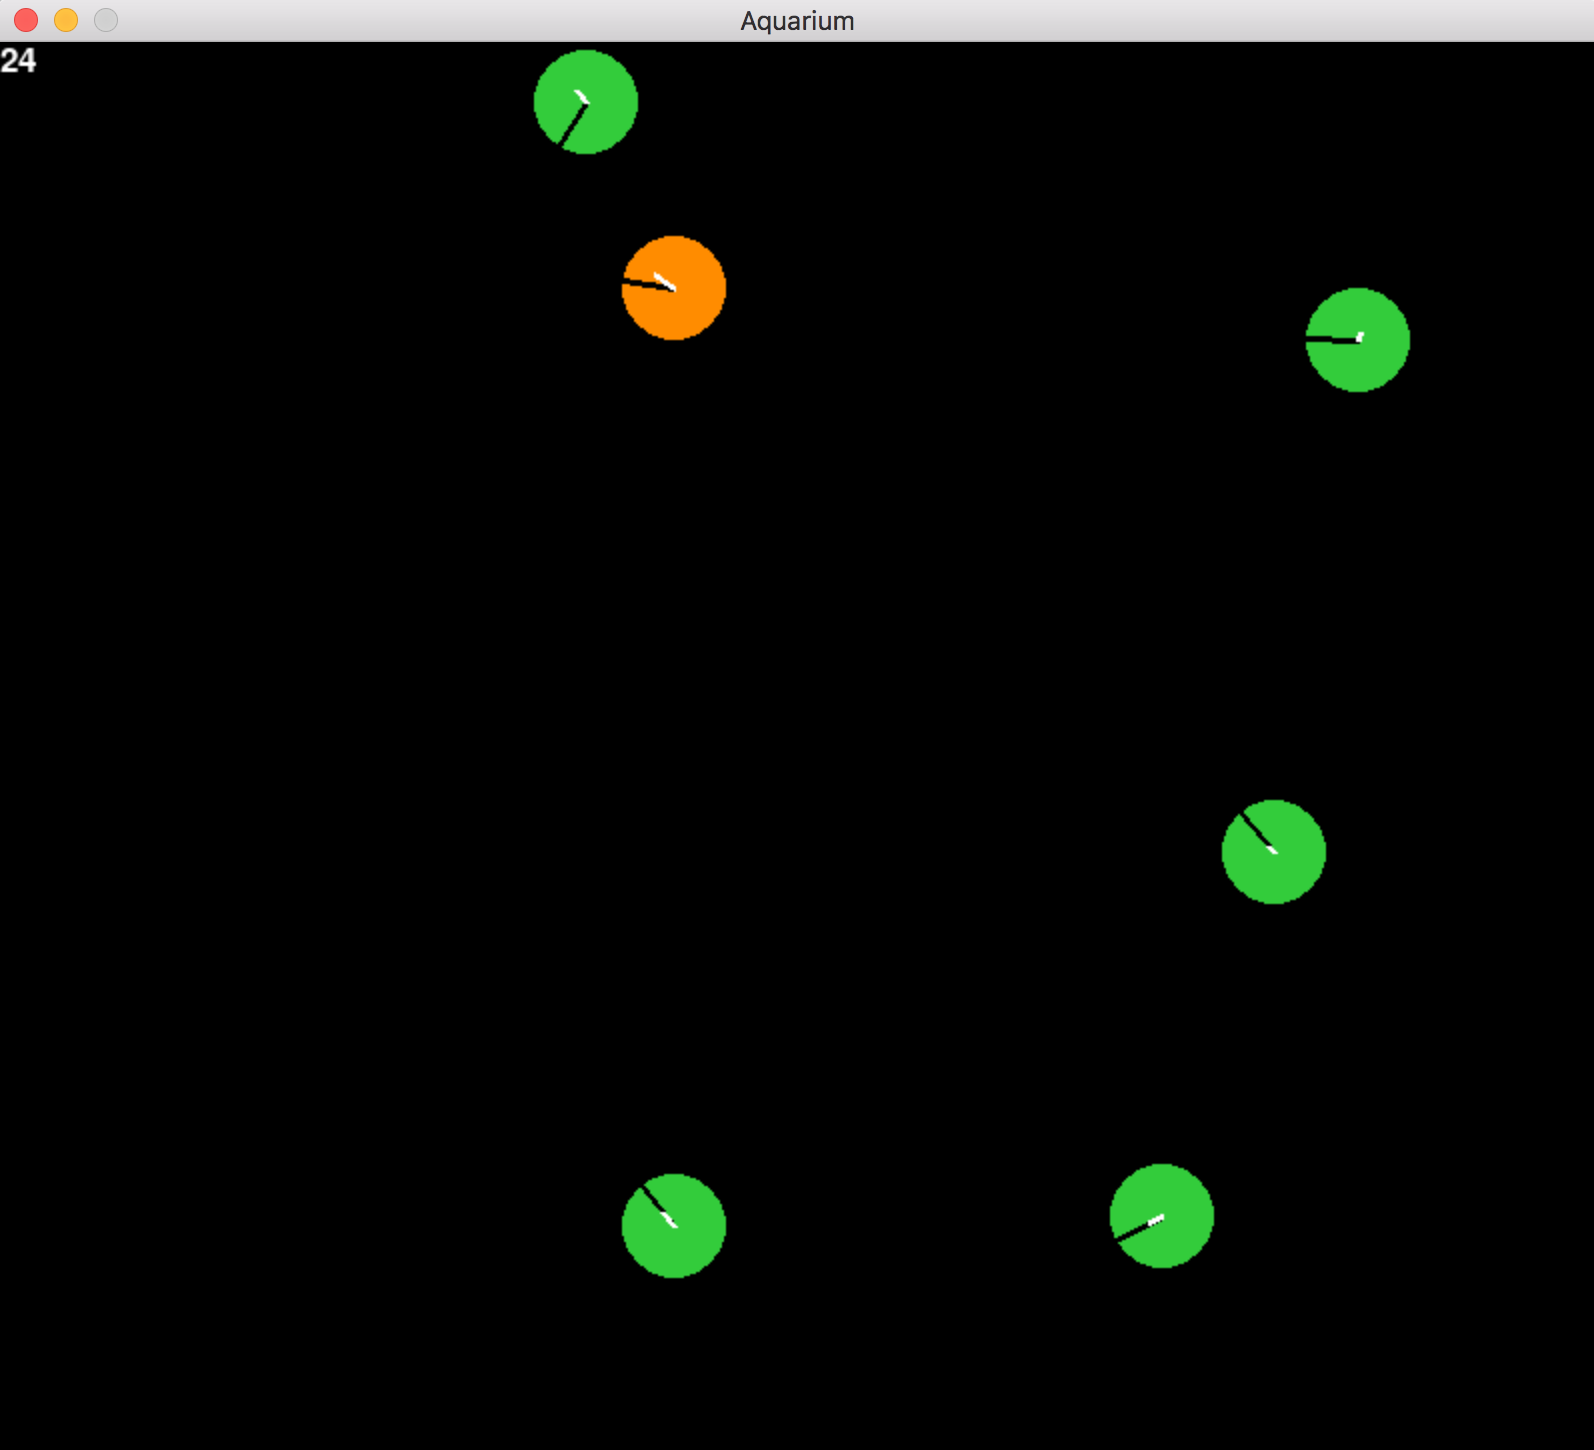
\includegraphics[width=\linewidth]{demo.png}
  \caption{The aquarium. Orange circle is a shark, green circles are fishes.}\label{fig:demo}
\end{figure}

Figure~\ref{fig:demo} shows an examplary simulation.

\subsection{Observation Space}

% TODO: Partial observability.

\subsection{Action Space}

\end{document}
